% Chapter 10

\chapter{Edge states and cross over} % Main chapter title

\label{Chapter10} % For referencing the chapter elsewhere, use \ref{Chapter9} 

\lhead{Part III. \emph{Two wires}}
\chead{Chapter 10. \emph{Edge states \& cross over}} % This is for the header on each page - perhaps a shortened title

%----------------------------------------------------------------------------------------
In this chapter we analyse the cross over from $p$- to $s$-wave pairing. We start with an analysis of the edge states in section \ref{sec.2wiresedgestatesedgestates}. We use this, along with Kramers degeneracy investigated in section \ref{sec.2wireskramersdegeneracy}, to analyse how the cross over happens qualitatively in section \ref{sec.2wirestransitionqualitative}. This is put on a firm footing by directly calculating the topogical invariants in section \ref{sec.2wires_CSinv}. In section \ref{sec.2wiresCrossover_energy} we analyse the cross over numerically and compare this to the expectation from the topological analysis of the previous sections. Finally in section \ref{sec.2wires_crossover_control_coherence_length} we discuss how the cross over can be controlled using the BEC coherence length rather than adjusting the actual interwire distance. 

\section{Edge states, separated wires}
\label{sec.2wiresedgestatesedgestates}
In this section we come with an approximate analytical solution for the edge states for the separated wires. This is done for a later discussion on their properties.

For the separated wires we have $\Delta^{12}_k = 0$. Analogously to the approach in section \ref{sec.edgestates} we can then write up a real space mean field Hamiltonian:
\begin{equation}
H_{FF} = \frac{1}{2}\int dx \Psi^\dagger_{F}(x) \mathcal{H}_{FF}(x) \Psi_{F}(x), \hspace{0.5cm} \mathcal{H}_{FF}(x) = \left(\frac{p^2}{2m_F} - \mu(x)\right)\sigma_0\otimes \tau_3 + \Delta^{11}(p)\sigma_3\otimes \tau_1.
\label{eq.2wiresMFHamiltonianrealspace}
\end{equation}
with $\Psi^\dagger_{F}(x) = \begin{bmatrix} \psi^\dagger_{1,F}(x) & \psi_{1,F}(x) & \psi^\dagger_{2,F}(x) & \psi_{2,F}(x)\end{bmatrix}$. Here we assume that $\mu = \mu(x)$ as shown in figure \ref{fig.edgestatesmux}. $\sigma_i$ and $\tau_i$ are the Pauli matrices in wire space and particle-hole space respectively. $p = -i\partial_x$ is the momentum operator in real space. The operator $\Delta^{11}(p)$ is defined by: $\Delta^{11}(p)\text{e}^{ikx} = \Delta^{11}_k\text{e}^{ikx}$. We have also dropped the grand energy $E_0$. We hereby get four edge state solutions to $\mathcal{H}_{FF}(x)\psi(x) = 0$. By keeping only $p$ up to first order as in section \ref{sec.edgestates} we get the approximate solutions:
\begin{align}
\psi^1_1(x) &= g_1(x)\text{e}^{i\pi/4}\chi^{3}_1\otimes\chi^{2}_2, \hspace{0.5cm} \psi^1_2(x) = g_2(x)\text{e}^{i\pi/4}\chi^{3}_1\otimes\chi^{2}_2, \nonumber \\
\psi^2_1(x) &= g_1(x)\text{e}^{-i\pi/4}\chi^{3}_2\otimes\chi^{2}_1, \hspace{0.5cm} \psi^2_2(x) = g_2(x)\text{e}^{-i\pi/4}\chi^{3}_2\otimes\chi^{2}_1,
\end{align}
with $\chi^{i}_a$ the $a$'th eigenvector to the $i$'th Pauli matrix. Explicitly: 
\begin{equation}
\chi^{3}_1 = \begin{bmatrix} 1 \\ 0 \end{bmatrix},  \hspace{0.5cm} \chi^{3}_1 = \begin{bmatrix} 0 \\ 1 \end{bmatrix}, \hspace{0.5cm} \chi^2_1 = \frac{1}{\sqrt{2}}\begin{bmatrix} 1 \\ i \end{bmatrix}, \hspace{0.5cm} \chi^2_2 = \frac{1}{\sqrt{2}}\begin{bmatrix} 1 \\ -i \end{bmatrix}. \nonumber
\end{equation}
Further: $g_1(x) = \frac{1}{N}\text{e}^{-\frac{1}{\Delta}\int_{0}^{x} dx' \mu(x')}$, $g_2(x) = \frac{1}{N}\text{e}^{-\frac{1}{\Delta}\int_{\mathcal{L}}^{x} dx' \mu(x')}$ and $N^2 = \frac{1}{2}\int dx |g_j(x)|^2$ is a normalization constant.

From equation \eqref{eq.2wiresTminuswireexchangefirstquantization} we have, that the time reversal operator that squares to minus the identity is given by: $\mathcal{T}_- = i\sigma_2\otimes\tau_0 \cdot K$. We hereby get: $\mathcal{T}_-\psi^1_1(x) = -\psi^2_1(x), \mathcal{T}_-\psi^1_2(x) = +\psi^2_2(x)$. The states belonging to separate wires are therefore Kramers partners. This is crucial for the following analysis. For sake of completeness let us write up the second quantized version of the four states above: 
\begin{align}
\gamma^1_{0,1} &= \int dx \; g_1(x)\frac{\text{e}^{i\pi/4}}{\sqrt{2}}(\psi_{1,F}(x)-i\psi^\dagger_{1,F}(x)), \hspace{0.5cm} \gamma^1_{0,2} = \int dx \; g_2(x)\frac{\text{e}^{i\pi/4}}{\sqrt{2}}(\psi_{1,F}(x)-i\psi^\dagger_{1,F}(x)), \nonumber \\
\gamma^2_{0,1} &= \int dx \; g_1(x)\frac{\text{e}^{-i\pi/4}}{\sqrt{2}}(\psi_{2,F}(x)+i\psi^\dagger_{2,F}(x)), \hspace{0.5cm} \gamma^2_{0,2} = \int dx \; g_2(x)\frac{\text{e}^{-i\pi/4}}{\sqrt{2}}(\psi_{2,F}(x) + i \psi^\dagger_{2,F}(x)). \nonumber 
\end{align}
Finally this yields the Kramers partners of fermionic annihilation operators:
\begin{align}
d_1 &= \frac{\gamma^1_{0,1} + i \gamma^1_{0,2}}{2} = \int dx\; g(x)\frac{\text{e}^{i\pi/4}}{\sqrt{2}}(\psi_{1,F}(x)-i\psi^\dagger_{1,F}(x)), \nonumber \\
d_2 &= \frac{\gamma^2_{0,1} + i \gamma^2_{0,2}}{2} = \int dx\; g(x)\frac{\text{e}^{-i\pi/4}}{\sqrt{2}}(\psi_{2,F}(x)+i\psi^\dagger_{2,F}(x)),
\label{eq.2wiresedgestatesannihilationoperators}
\end{align}
with $g(x) = (g_1(x) + ig_2(x))/2$. That they are Kramers partners means that $T_-d_1T_-^{-1} = d_2$. 

\section{Kramers degeneracy: protection of edge states}
\label{sec.2wireskramersdegeneracy}
In this section we show, that the interwire interaction protects the edge states as long as no interwire mean field has formed. We show, that this is because Kramers partners do not couple.

Consider a general system described by the Hamiltonian $H$. Assume, that this Hamiltonian is time reversal invariant, $[T, H] = 0$, and that $T^2 = -\mathbb{I}$. Let $\ket{\psi_1}$ and $\ket{\psi_2}$ be eigenstates to the Hamiltonian, with energy $E_1$ and $E_2$, and Kramers partners: $\ket{\psi_2} = T\ket{\psi_1}$. Since $[T, H] = 0$ the two states have the same energy: 
\begin{equation}
E_2\ket{\psi_2} = HT\ket{\psi_1} = TH\ket{\psi_1} = E_1\ket{\psi_2}. \nonumber
\end{equation}
So $E_2 = E_1$. Further, the states are orthogonal:
\begin{equation}
\braket{\psi_1|\psi_2} = \braket{T\psi_2|T\psi_1} = \braket{-\psi_1|\psi_2} = -\braket{\psi_1|\psi_2} \Rightarrow \braket{\psi_1|\psi_2} = 0. \nonumber  
\end{equation}
In the first equality we use, that we can flip the inner product by going to the time reversed states \cite[p. 274]{Sakurai}. In the second equality we use, that $T\ket{\psi_2} = -\ket{\psi_1}$, since $T^2 = -\mathbb{I}$. Hence, any energy state in a time reversal invariant system with $T^2 = -\mathbb{I}$ is twofold degenerate. This is Kramers degeneracy. Now let $H'$ be a perturbation to the Hamiltonian, which respects the time reversal symmetry: $[T, H'] = 0$. In degenerate perturbation theory we calculate the matrix with entries $W_{ij} = \bra{\psi_i}H'\ket{\psi_j}$. The eigenstates of $H$ remain good eigenstates if the states uncouple: $\bra{\psi_1}H'\ket{\psi_2} = 0$, so that $W_{ij}$ is diagonal. This is exactly the case for Kramers partners: 
\begin{equation}
\bra{\psi_1}H'\ket{\psi_2} = \bra{T\psi_2}TH'T^{-1}\ket{T\psi_1} = \bra{T\psi_2}H'\ket{T\psi_1} = -\bra{\psi_1}H'\ket{\psi_2} \Rightarrow \bra{\psi_1}H'\ket{\psi_2} = 0. \nonumber
\end{equation}
The first equality holds, since $H'$ is hermitian \cite{Sakurai}. 

Now what has this to do with the system at hand? We let $\ket{\psi_j} = d^\dagger_j\ket{\text{S}}_0$ for $j = 1, 2$. If we can show, that the interwire interaction $H' = H^\text{int}_{FF,12}$ is time reversal invariant under $T_-$, then the above analysis shows that the edge states cannot couple. From equation \eqref{eq.Hint12realspace} we have:
\begin{equation}
H^\text{int}_{FF,12} = \int dx_1 dx_2 \psi^\dagger_{1,F}(x_1)\psi^\dagger_{2,F}(x_2) \tilde{V}_{\text{ind}}^{12}(x_1-x_2,0) \psi_{2,F}(x_2)\psi_{1,F}(x_1),
\end{equation}
with $\tilde{V}_{\text{ind}}^{12}(x_1-x_2,0)$ the zero frequency induced interaction in real space. Now $T_-\psi_{1,F}(x)T^{-1}_- = \psi_{2,F}(x)$ and $T_-\psi_{2,F}(x)T^{-1}_- = -\psi_{1,F}(x)$. Finally, $\tilde{V}_{\text{ind}}^{12}(x, 0)$ is real, so we get that $T_-H^\text{int}_{FF,12}T_-^{-1} = H^\text{int}_{FF,12}$. Hence, the edge states does not couple through the interwire interaction. Therefore they are protected, as long as the interwire interaction is a perturbation to the system, which is to say no interwire mean field has formed.  

\section{Qualitative understanding of cross over}
\label{sec.2wirestransitionqualitative}
In this section we come with a qualitative analysis of how the cross over from $p$- to $s$-wave occures using the previous two sections. 

We can qualitatively understand the two ways in which the cross over from $p$- to $s$-wave pairing occures as follows. 

\textbf{Imaginary interwire pairing}: Assume that as the wires are brought closer together, the system chooses the interwire pairing to be \textit{imaginary}. Then the system \textit{breaks} the time reversal symmetry $T_-$. In this case there is no longer a Kramers degeneracy. As a consequence the edge states can couple and gap away. We can actually calculate by how much the edge states gap. In this connection we define the operator $\Delta^{12}(p)$ as: $\Delta^{12}(p)\text{e}^{ikx} = \Delta^{12}_k\text{e}^{ikx}$. Since $\Delta^{12}_k$ is even in $k$, there is no first order term in $k$. Hence for states with small curvatures like the edge states we can approximate $\Delta^{12}(p) = \Delta^{12}_{k=0}$. This means, that the perturbation in real space relevant for the edge states is:
\begin{equation}
\mathcal{H}'_{FF}(x) = \Delta^{12}_{k=0} \sigma_2\otimes \tau_1. 
\label{eq.interwirepairingrealspace}
\end{equation}
The edge states in wires 1 and 2 in first quantization are described by the wave functions:
\begin{equation}
\psi_1(x) = \frac{1}{2}(\psi^1_1(x) + i\psi^1_2(x)) = g(x)\text{e}^{i\pi/4}\chi^3_1\otimes\chi^2_2, \hspace{0.5cm} \psi_2(x) = \frac{1}{2}(\psi^2_1(x) + i\psi^2_2(x)) = g(x)\text{e}^{-i\pi/4}\chi^3_2\otimes\chi^2_1. \nonumber
\end{equation} 
Hence the coupling is given by:
\begin{align}
\bra{\psi_1}\mathcal{H}'_{FF}\ket{\psi_2} &= \Delta^{12}_{k=0}\text{e}^{-i\pi/2}\bra{\chi^3_1\otimes\chi^2_2}\sigma_2\otimes \tau_1\ket{\chi^3_2\otimes\chi^2_1}\int dx \; |g(x)|^2 = -i\Delta^{12}\braket{\chi^3_1\otimes\chi^2_2 | \chi^3_1\otimes\chi^2_2} \nonumber \\
 &= -i\Delta^{12}_{k=0}. \nonumber
\end{align}
Further, $\mathcal{H}'_{FF}$ only couples states belonging to separate wires. Hence the diagonal elements vanish: $\bra{\psi_j}\mathcal{H}'_{FF}\ket{\psi_j} = 0$. So the perturbation matrix is:
\begin{equation}
W = \begin{bmatrix} 0 & -i\Delta^{12}_{k=0} \\ i\Delta^{12}_{k=0} & 0 \end{bmatrix}. \nonumber
\end{equation}
The energy shifts of the states are then simply $\pm \Delta^{12}_{k=0}$. This makes it explicit, how the states are gapped! This is the content of figure \ref{fig.2wiresedgestates} going from the top center to the middle left. 

\textbf{Real interwire pairing}: Assume that as the wires are brought closer together, the system chooses the interwire pairing to be \textit{real}. In this situation the system still respects the time reversal symmetry $T_-$. Kramers degeneracy is still present and therefore any energy state must be twofold degenerate. Further, since the system has a particle-hole symmetry the energy spectrum is symmetric around $E = 0$ (relative to the ground state). Therefore the zero energy edge states are locked as long as the bulk energy gap remains open. A direct calculation of the first order energy shift performed in the same way as in the above verifies this explicitly. The bulk energy dispersions in this situation are given by: $E^{\pm}_{F,k} = \sqrt{\varepsilon^2_k + (\Delta^{11}_k \pm \Delta^{12}_k)^2}$. The bulk gap will therefore eventually close as we bring the wires closer together. This happens exactly when $|\Delta^{12}_{k_0}| = |\Delta^{11}_{k_0}|$, where $\pm k_0$ are the Fermi points given by: $\varepsilon_{\pm k_0} = 0$. Hence, we expect a topological phase transition in this situation, with a topologically non-trivial system for $|\Delta^{12}_{k_0}| < |\Delta^{11}_{k_0}|$ and topologically trivial for $|\Delta^{12}_{k_0}| > |\Delta^{11}_{k_0}|$. This is the content of figure \ref{fig.2wiresedgestates} going from the top center to the middle and bottom right. 

\begin{figure}
\center
\begin{tikzpicture}
\draw[|-latex, thick] (0, 0) -- (0,  2) node[above]{$E$};
\draw[-, thick]   (0, 0) -- (0, -2);
\node at (-0.4, 0) {$0$};

\draw[-, dashed] (0, 1)--(2, 1);
\draw[-, thick] (-0.1, 1)--(0.1, 1);
\node at (-0.7,1) {$E_{F,k_0}$};

\draw[-, dashed] (0,    -1) -- (2,   -1);
\draw[-, thick]  (-0.1, -1) -- (0.1, -1);
\node at (-0.85,-1) {$-E_{F,k_0}$};

\draw[-, ultra thick] (1, 1)--(1, 2);
\draw[-, ultra thick] (1, -1)--(1, -2);
\node[red] at (1, 0) {\textbullet};

\draw[-, ultra thick] (2, 1)--(2, 2);
\draw[-, ultra thick] (2, -1)--(2, -2);
\node[blue] at (2, 0) {\textbullet};

\draw[-, dashed] (0,0.01) -- (2,0.01);

\node at (3, -1.9) {$0$};
\node at (5, -1.9) {$\mathcal{L}$};

\draw[scale=0.5,domain=-1:1,smooth,variable=\x,red] plot ({\x + 6},{ 2 * exp{- 15 * \x*\x} - 3});
\draw[scale=0.5,domain=-1:1,smooth,variable=\x,red] plot ({\x + 10},{ 2 * exp{- 15 * \x*\x} -3});
\draw[|-latex, thick ] (3,-1.5) -- (5.8,-1.5) node[right]{$x$};
\draw[-, ultra thick ] (3,-1.5) -- (5,-1.5);

\node at (3, 1.1) {$0$};
\node at (5, 1.1) {$\mathcal{L}$};

\draw[scale=0.5,domain=-1:1,smooth,variable=\x,blue] plot ({\x + 6},{ 2 * exp{- 15 * \x*\x} + 3});
\draw[scale=0.5,domain=-1:1,smooth,variable=\x,blue] plot ({\x + 10},{ 2 * exp{- 15 * \x*\x} + 3});

\draw[|-latex, thick ] (3,1.5) -- (5.8,1.5) node[right]{$x$};
\draw[-, ultra thick] (3, 1.5) -- (5, 1.5);

%\draw[-, dashed] (5.8, -1.5) -- (5.8, 1.5);
\node at (2.2, 2.8) {$\Delta^{12}_k = 0$};

%%%%%%%%%%%%%%%%%%%%%%%%%%%%%%%%%%%
\pgfmathsetmacro{\hmove}{-4}
\pgfmathsetmacro{\vmove}{-6}

\draw[|-latex, thick] (\hmove, \vmove) -- (\hmove,  2 + \vmove) node[above]{$E$};
\draw[-, thick]   (\hmove, \vmove) -- (\hmove, -2 + \vmove);
\node at (-0.4 + \hmove, 0 + \vmove) {$0$};

\draw[-, dashed] (0 + \hmove, 1 + \vmove)--(2 + \hmove, 1 + \vmove);
\draw[-, thick] (-0.1 + \hmove, 1 + \vmove)--(0.1 + \hmove, 1 + \vmove);
\node at (-0.7 + \hmove, 1 + \vmove) {$E_{F,k_0}$};

\draw[-, dashed] (0 + \hmove,    -1 + \vmove) -- (2 + \hmove,   -1 + \vmove);
\draw[-, thick]  (-0.1 + \hmove, -1 + \vmove) -- (0.1 + \hmove, -1 + \vmove);
\node at (-0.85 + \hmove,-1 + \vmove) {$-E_{F,k_0}$};

\draw[-, ultra thick] (1 + \hmove, 1 + \vmove)--(1 + \hmove, 2 + \vmove);
\draw[-, ultra thick] (1 + \hmove, -1 + \vmove)--(1 + \hmove, -2 + \vmove);

%gapped edge state:
\coordinate (edge1energy) at (1 + \hmove, 0.5 + \vmove);
\node[right=0.0cm of edge1energy] {$+\Delta^{12}_{k=0}$}; 
\draw[-latex, semithick] (1 + \hmove, 0 + \vmove)--(1 + \hmove, 0.5 + \vmove);
\node[red] at (edge1energy) {\textbullet};

\draw[-, ultra thick] (2 + \hmove, 1 + \vmove)--(2 + \hmove, 2 + \vmove);
\draw[-, ultra thick] (2 + \hmove, -1 + \vmove)--(2 + \hmove, -2 + \vmove);

%gapped edge state:
\coordinate (edge2energy) at (2 + \hmove, -0.5 + \vmove);
\node[right=0.0cm of edge2energy] {$-\Delta^{12}_{k=0}$}; 
\draw[-latex, semithick] (2 + \hmove, 0 + \vmove)--(2 + \hmove, -0.5 + \vmove);
\node[blue] at (edge2energy) {\textbullet};

\draw[-, dashed] (0 + \hmove,0.01 + \vmove) -- (2 + \hmove,0.01 + \vmove);

\node at (3 + \hmove, -1.4 + \vmove) {$0$};
\node at (5 + \hmove, -1.4 + \vmove) {$\mathcal{L}$};

\draw[|-latex, thick ] (3 + \hmove,-1.0 + \vmove) -- (5.8 + \hmove,-1.0 + \vmove) node[right]{$x$};
\draw[-, ultra thick ] (3 + \hmove,-1.0 + \vmove) -- (5 + \hmove,-1.0 + \vmove);

\node at (3 + \hmove, 0.6 + \vmove) {$0$};
\node at (5 + \hmove, 0.6 + \vmove) {$\mathcal{L}$};

\draw[|-latex, thick ] (3 + \hmove, 1.0 + \vmove) -- (5.8 + \hmove,1.0 + \vmove) node[right]{$x$};
\draw[-, ultra thick] (3 + \hmove, 1.0 + \vmove) -- (5 + \hmove, 1.0 + \vmove);

\node at (2.2 + \hmove, 2.8 + \vmove) {$\Delta^{12}_k \neq 0$, imaginary};

%%%%%%%%%%%%%%%%%%%%%%%%%%%%%%%%%%%
\pgfmathsetmacro{\hmove}{4}
\pgfmathsetmacro{\vmove}{-6}
\pgfmathsetmacro{\Eminchange}{0.4}

\draw[|-latex, thick] (\hmove, \vmove) -- (\hmove,  2 + \vmove) node[above]{$E$};
\draw[-, thick]   (\hmove, \vmove) -- (\hmove, -2 + \vmove);
\node at (-0.4 + \hmove, 0 + \vmove) {$0$};

\draw[-, dashed] (0 + \hmove, 1 - \Eminchange + \vmove)--(2 + \hmove, 1 - \Eminchange + \vmove);
\draw[-, thick] (-0.1 + \hmove, 1 - \Eminchange + \vmove)--(0.1 + \hmove, 1 - \Eminchange + \vmove);
\node at (-0.7 + \hmove, 1 - \Eminchange + \vmove) {$E_{F,k_0}$};

\draw[-, dashed] (0 + \hmove,    -1 + \Eminchange + \vmove) -- (2 + \hmove,   -1 + \Eminchange + \vmove);
\draw[-, thick]  (-0.1 + \hmove, -1 + \Eminchange + \vmove) -- (0.1 + \hmove, -1 + \Eminchange + \vmove);
\node at (-0.85 + \hmove, -1 + \Eminchange + \vmove) {$-E_{F,k_0}$};

\draw[-, ultra thick] (1 + \hmove, 1 - \Eminchange + \vmove)--(1 + \hmove, 2 + \vmove);
\draw[-, ultra thick] (1 + \hmove, -1 + \Eminchange + \vmove)--(1 + \hmove, -2 + \vmove);
\node[red] at (1 + \hmove, 0 + \vmove) {\textbullet};

\draw[-, ultra thick] (2 + \hmove, 1 - \Eminchange + \vmove)--(2 + \hmove, 2 + \vmove);
\draw[-, ultra thick] (2 + \hmove, -1 + \Eminchange + \vmove)--(2 + \hmove, -2 + \vmove);
\node[blue] at (2 + \hmove, 0 + \vmove) {\textbullet};

\draw[-, dashed] (0 + \hmove, 0.01 + \vmove) -- (2 + \hmove, 0.01 + \vmove);

\node at (3 + \hmove, -1.4 + \vmove) {$0$};
\node at (5 + \hmove, -1.4 + \vmove) {$\mathcal{L}$};

\draw[scale=0.5,domain=-1:1,smooth,variable=\x,red] plot ({\x + 6 + 2*\hmove},{ 2 * exp{- 15 * \x*\x} - 2.0 + 2*\vmove});
\draw[scale=0.5,domain=-1:1,smooth,variable=\x,red] plot ({\x + 10 + 2*\hmove},{ 2 * exp{- 15 * \x*\x} -2.0 + 2*\vmove});
\draw[|-latex, thick ] (3 + \hmove,-1.0 + \vmove) -- (5.8 + \hmove,-1.0 + \vmove) node[right]{$x$};
\draw[-, ultra thick ] (3 + \hmove,-1.0 + \vmove) -- (5 + \hmove,-1.0 + \vmove);

\node at (3 + \hmove, 0.6 + \vmove) {$0$};
\node at (5 + \hmove, 0.6 + \vmove) {$\mathcal{L}$};

\draw[scale=0.5,domain=-1:1,smooth,variable=\x,blue] plot ({\x + 6  + 2*\hmove},{ 2 * exp{- 15 * \x*\x} + 2.0 + 2*\vmove});
\draw[scale=0.5,domain=-1:1,smooth,variable=\x,blue] plot ({\x + 10 + 2*\hmove},{ 2 * exp{- 15 * \x*\x} + 2.0 + 2*\vmove});

\draw[|-latex, thick ] (3 + \hmove,1.0 + \vmove) -- (5.8 + \hmove,1.0 + \vmove) node[right]{$x$};
\draw[-, ultra thick] (3 + \hmove, 1.0 + \vmove) -- (5 + \hmove, 1.0 + \vmove);

\node at (2.2 + \hmove, 2.8 + \vmove) {$|\Delta^{12}_{k_0}| < |\Delta^{11}_{k_0}|$, real};

%squezzing of gap:
\draw[-latex, semithick] (0.5 + \hmove, 1  + \vmove)--(0.5 + \hmove, 1 - \Eminchange + \vmove);
\draw[-latex, semithick] (0.5 + \hmove, -1 + \vmove)--(0.5 + \hmove, -1 + \Eminchange + \vmove);

%%%%%%%%%%%%%%%%%%%%%%%%%%%%%%%%%%%
\pgfmathsetmacro{\hmove}{4}
\pgfmathsetmacro{\vmove}{-12}
\pgfmathsetmacro{\Eminchange}{0.4}

\draw[|-latex, thick] (\hmove, \vmove) -- (\hmove,  2 + \vmove) node[above]{$E$};
\draw[-, thick]   (\hmove, \vmove) -- (\hmove, -2 + \vmove);
\node at (-0.4 + \hmove, 0 + \vmove) {$0$};

\draw[-, dashed] (0 + \hmove, 1 - \Eminchange + \vmove)--(2 + \hmove, 1 - \Eminchange + \vmove);
\draw[-, thick] (-0.1 + \hmove, 1 - \Eminchange + \vmove)--(0.1 + \hmove, 1 - \Eminchange + \vmove);
\node at (-0.7 + \hmove, 1 - \Eminchange + \vmove) {$E_{F,k_0}$};

\draw[-, dashed] (0 + \hmove,    -1 + \Eminchange + \vmove) -- (2 + \hmove,   -1 + \Eminchange + \vmove);
\draw[-, thick]  (-0.1 + \hmove, -1 + \Eminchange + \vmove) -- (0.1 + \hmove, -1 + \Eminchange + \vmove);
\node at (-0.85 + \hmove, -1 + \Eminchange + \vmove) {$-E_{F,k_0}$};

\draw[-, ultra thick] (1 + \hmove, 1 - \Eminchange + \vmove)--(1 + \hmove, 2 + \vmove);
\draw[-, ultra thick] (1 + \hmove, -1 + \Eminchange + \vmove)--(1 + \hmove, -2 + \vmove);
%\node[red] at (1 + \hmove, 0 + \vmove) {\textbullet};

\draw[-, ultra thick] (2 + \hmove, 1 - \Eminchange + \vmove)--(2 + \hmove, 2 + \vmove);
\draw[-, ultra thick] (2 + \hmove, -1 + \Eminchange + \vmove)--(2 + \hmove, -2 + \vmove);
%\node[blue] at (2 + \hmove, 0 + \vmove) {\textbullet};

\draw[-, dashed] (0 + \hmove, 0.01 + \vmove) -- (2 + \hmove, 0.01 + \vmove);

\node at (3 + \hmove, -0.9 + \vmove) {$0$};
\node at (5 + \hmove, -0.9 + \vmove) {$\mathcal{L}$};

\draw[|-latex, thick ] (3 + \hmove,-0.5 + \vmove) -- (5.8 + \hmove,-0.5 + \vmove) node[right]{$x$};
\draw[-, ultra thick ] (3 + \hmove,-0.5 + \vmove) -- (5 + \hmove,  -0.5 + \vmove);

\node at (3 + \hmove, 0.1 + \vmove) {$0$};
\node at (5 + \hmove, 0.1 + \vmove) {$\mathcal{L}$};

\draw[|-latex, thick ] (3 + \hmove,0.5 + \vmove) -- (5.8 + \hmove,0.5 + \vmove) node[right]{$x$};
\draw[-, ultra thick] (3 + \hmove, 0.5 + \vmove) -- (5 + \hmove,  0.5 + \vmove);

\node at (2.2 + \hmove, 2.8 + \vmove) {$|\Delta^{12}_{k_0}| > |\Delta^{11}_{k_0}|$, real};

%squezzing of gap:
\draw[-latex, semithick] (0.5 + \hmove, 1 - \Eminchange + \vmove)--(0.5 + \hmove, 1  + \vmove);
\draw[-latex, semithick] (0.5 + \hmove, -1 + \Eminchange + \vmove)--(0.5 + \hmove, -1 + \vmove);

\end{tikzpicture}
\caption{Top centered: for $\Delta^{12}_k=0$ we have two copies of the single wire system with the interwire interaction as a perturbation. There are two symmetry-protected edge states, one at each wire and two energy dispersions mirrored in $E = 0$. This is indicated with red and blue dots. $k_0$ is defined by: $0 = \varepsilon_{k_0} = \frac{k^2_0}{2m_F} - \mu$. Middle left: If the system chooses an imaginary interwire pairing the system breaks the $T^2 = -\mathbb{I}$ symmetry. The edge states are therefore no longer protected at $E = 0$, and the edge states are gapped by $2\Delta^{12}_{k=0}$. Middle and bottom right: If the system chooses a real interwire pairing the system still respects the $T^2 = -\mathbb{I}$ symmetry. Middle right: Before an energy gap closing the edge states are still protected. The gap is closing; this is indicated by the arrows squezzing the gap. Bottom right: After the gap closing the edge states are gone. The system is topologically trivial. The gap is opening again indicated by the arrows.}
\label{fig.2wiresedgestates}
\end{figure}


\section{Chern-Simons invariants}
\label{sec.2wires_CSinv}
In this section we directly calculate the Chern-Simons topological invariant for the two wire system. This is to bring the considerations of the previous section on a firm footing. In turn we calculate the Wilson loop and use this to characterize the system topologically. 

The Berry connection for a system with several negative energy states becomes a matrix:
\begin{equation}
\mathcal{A}^{ij}_k = \bra{e^{-}_{i,k}}\partial_k\ket{e^{-}_{j,k}}.
\end{equation}
In the present case the Berry connection is a $2\times 2$ matrix. In the case of a $T^2 = + \mathbb{I}$ symmetry the topological invariant, $\nu$, is calculated in analogy to the one in section \ref{sec.CS1} and is given by the twice the Chern-Simons invariant:
\begin{align}
\nu_{\mathbb{Z}} &= 2\text{CS}_1 = \frac{i}{\pi} \int dk\; \text{tr}[\mathcal{A}] = \frac{i}{\pi} \int dk\; \left[\bra{e^{-}_{1,k}}\partial_k\ket{e^{-}_{1,k}} + \bra{e^{-}_{2,k}}\partial_k\ket{e^{-}_{2,k}}  \right] \nonumber \\
 &= 2(\text{CS}_{1,1} + \text{CS}_{1,2})\in \mathbb{Z}, \hspace{0.5cm} T^2 = +\mathbb{I}.
\label{eq.2wires.topinv.T2eqplus1}
\end{align}
Here we have indicated the contribution to the Chern-Simons invariant from the eigenvector $\ket{e^{-}_{i,k}}$ with $\text{CS}_{1,i}$. We will refer to these as the subsystem invariants. For $T^2 = +\mathbb{I}$ the subsystem invariants are not well-defined, only their sum is. For $T^2 = -\mathbb{I}$, Kramers degeneracy means, that as long as one Kramers partner is protected, so is the other. Since $\ket{e^{-}_{1,k}}$ and $\ket{e^{-}_{2,k}}$ are the only available eigenvectors to negative eigenvalues, these must be Kramers partners.\footnote{This can also be verified explicitly}. Hence, the topological invariant is found by simply calculated either $\text{CS}_{1,1}$ or $\text{CS}_{1,2}$\cite{FuKane2006, LiYangChen} and \cite[pp. 130-135]{BernevigTITSC}. In turns out, that the $\mathbb{Z}_2$ invariant can then be calculated by going to the Wilson loop:
\begin{equation}
\nu_{\mathbb{Z}_2} = W_{1,1} = \text{e}^{2\pi i\text{CS}_{1,1}} = \pm 1, \hspace{0.5cm} T^2 = -\mathbb{I}.
\label{eq.2wires.topinv.T2eqminus1}
\end{equation}
We are now ready for the computation. This will be done in the two cases $\Delta^{12}_k$ imaginary and real corresponding to the presence of a wire exchanging time reversal symmetry of the form $T^2 = +\mathbb{I}$ and $T^2 = -\mathbb{I}$ respectively. 

\subsection{Imaginary interwire pairing}
\label{subsec.2wires_CSinv_Delta12imag}
The aim of this subsection is to calculate $\nu_{\mathbb{Z}}$ as given in equation \eqref{eq.2wires.topinv.T2eqplus1}. We follow the same procedure as the one in section \ref{sec.CS1}. 

Since we differentiate the eigenvectors with respect to $k$, it is essential that these are well-behaved in any $k$. If we look closely at the eigenvectors derived back in section \ref{sec.2wiresgrandHFF}, we can see that if $\Delta^{12}_k = 0$, the eigenvectors are not well-behaved in $k = 0$. Back then this was no issue, since a single problem point in the integral makes no difference.\footnote{One might be concerned about this line of thinking. However, the gap equations in the special cases investigated in the current section have also been derived using well-behaved eigenvectors. The result is the same.} Hence, the single truly tricky part is to get well-behaved eigenvectors. However, there is a procedure for it, which was also used in section \ref{sec.CS1}. This procedure is described in \cite{Ryu.Topology}. First we transform the Hamiltonian to the standard Nambu spinor form, so that $C_k \to \tilde{C}_k = \begin{bmatrix} c_{1,k} & c_{2,k} & c^\dagger_{1,-k} & c^\dagger_{2,-k}  \end{bmatrix}^{T}$. This amounts to the following transformation of $\mathcal{H}_{FF,k}$:
\begin{align}
\mathcal{H}_{FF,k} &= \varepsilon_k \sigma_0 \otimes \tau_3 + \Delta^{11}_k \sigma_3 \otimes \tau_1 + \Delta^{12}_k \sigma_2 \otimes \tau_1 \to \nonumber \\
\mathcal{H}'_{FF,k} &= \varepsilon_k \sigma_3 \otimes \tau_0 + \Delta^{11}_k \sigma_1 \otimes \tau_3 + \Delta^{12}_k \sigma_1 \otimes \tau_2, \nonumber 
\end{align}
where $\otimes$ is the direct product, $\tau_i$ is the Pauli matrices in particle-hole space and $\sigma_i$ are the Pauli matrices in wire-space. We have also written the imaginary interwire pairing as $i\Delta^{12}_k$. Notice, that we simply flip the $\tau$ and $\sigma$ matrices. Since the Hamiltonian both has a time reversal and particle-hole symmetry, it also has a chiral symmetry: $\{\mathcal{S}, \mathcal{H}_{FF,k}\} = 0$. In the new basis after the above transformation we see, that $\mathcal{S} = \sigma_1\otimes \tau_1$. $\mathcal{S}$ has eigenvectors $v_{ab} = \chi^{1}_a\otimes \chi^{1}_b$, where $\chi^{1}_a$ for $a = 1,2$ are the eigenvectors to the first Pauli matrix $\tau_1, \sigma_1$. We then transform to the basis, where $\mathcal{S}$ is diagonal by forming $V = (v_{ab})$ and calculating:
\begin{equation}
\tilde{\mathcal{H}}_{FF,k} = V^\dagger\mathcal{H}'_{FF,k}V = \varepsilon_k \sigma_1\otimes \tau_1 + \Delta^{11}_k \sigma_1\otimes\tau_3 - \Delta^{12}_k\sigma_2\otimes\tau_0. \nonumber 
\end{equation}
We then get the eigenvectors to negative energy eigenvalues:
\begin{equation}
\ket{e^{-}_{1,k}} = \frac{1}{\sqrt{2}E_{F,k}}\begin{bmatrix} \varepsilon_k \\ -\Delta^{11}_k + i\Delta^{12}_k \\ 0 \\ -E_{F,k} \end{bmatrix}, \hspace{0.5cm} \ket{e^{-}_{2,k}} = \frac{1}{\sqrt{2}E_{F,k}}\begin{bmatrix} \Delta^{11}_k + i\Delta^{12}_k \\ \varepsilon_k \\  -E_{F,k} \\ 0 \end{bmatrix},
\end{equation}
with $E_{F,k} = \sqrt{\varepsilon_k^2 + (\Delta^{11}_k)^2 + (\Delta^{12}_k)^2}$. These eigenvectors are manifestly well-defined for all $k$. Using these we explicitly get:
\begin{equation}
\mathcal{A}^{11}_k = \bra{e^{-}_{1,k}}\partial_k\ket{e^{-}_{1,k}} = -\frac{i}{2E_{F,k}^2}(\Delta^{11}_k\partial_k\Delta^{12}_k - \Delta^{12}_k\partial_k\Delta^{11}_k) = -\mathcal{A}^{22}_k. \nonumber
\end{equation}
Hereby: $\text{tr}[\mathcal{A}_k] = \mathcal{A}^{11}_k  + \mathcal{A}^{22}_k = 0$, and the topological invariant is simply $\nu_{\mathbb{Z}} = 0$. As for the single wire this is the topologically trivial value. This means, that the edge states formed in the single wire are not protected in the two wire system, when we only have a time reversal symmetry with $T^2 = +\mathbb{I}$. This is consistent with the more pictorial analysis of the last section. 

\subsection{Real interwire pairing}
\label{subsec.2wires_CSinv_Delta12real}
For a real interwire pairing the system both has a $T^2 = +\mathbb{I}$ and $T^2=-\mathbb{I}$ symmetry. The former is given by $T_2$ of section \ref{subsec.TRseparatewires}, the latter by $T_-$ of section \ref{subsec.TRwireexchange}. Therefore, we calculate both the $\mathbb{Z}$ and $\mathbb{Z}_2$ invariant from equation \eqref{eq.2wires.topinv.T2eqplus1} and \eqref{eq.2wires.topinv.T2eqminus1} respectively.

To get to well-behaved eigenvectors we follow the same procedure as outlined in the previous subsection. The $\Delta^{12}_k$ term of $\mathcal{H}_{FF,k}$ now has the form $\Delta^{12}_k \sigma_2 \otimes \tau_2$. After going to the Nambu spinor form, we therefore have $\mathcal{H}'_{FF,k} = \varepsilon_k \sigma_3 \otimes \tau_0 + \Delta^{11}_k \sigma_1 \otimes \tau_3 + \Delta^{12}_k \sigma_2 \otimes \tau_2$. The anticommuting symmetry is now given by: $\mathcal{S} = \sigma_1\otimes \tau_2$. The corresponding eigenvectors are therefore $v_{ab} = \chi^{1}_a\otimes\chi^{2}_b$. Letting $V = (v_{ab})$ and calculating the conjugation of $\mathcal{H}'_{FF,k}$ then yields:
\begin{equation}
\tilde{\mathcal{H}}_{FF,k} = V^\dagger\mathcal{H}'_{FF,k}V = \varepsilon_k \sigma_1\otimes \tau_1 + \Delta^{11}_k \sigma_1\otimes\tau_3 - \Delta^{12}_k\sigma_2\otimes\tau_1. \nonumber 
\end{equation}
To calculate the $\mathbb{Z}$ topological invariant, we need both negative energy eigenvectors:
\begin{equation}
\ket{e^{-}_{1,k}} = \frac{1}{2E^{+}_{F,k}}\begin{bmatrix} \varepsilon_k + i(\Delta^{11}_k + \Delta^{12}_k) \\ i(\varepsilon_k + i(\Delta^{11}_k + \Delta^{12}_k)) \\ -iE^{+}_{F,k} \\ -E^{+}_{F,k} \end{bmatrix}, \hspace{0.5cm} \ket{e^{-}_{2,k}} = \frac{1}{2E^{-}_{F,k}}\begin{bmatrix} \varepsilon_k + i(-\Delta^{11}_k + \Delta^{12}_k) \\ -i(\varepsilon_k + i(-\Delta^{11}_k + \Delta^{12}_k)) \\ iE^{-}_{F,k} \\ -E^{-}_{F,k} \end{bmatrix}. \nonumber
\end{equation}
These are seen to be manifestly well-defined for all $k$. Since the entries of $\ket{e^{-}_{1,k}}$ and $\ket{e^{-}_{2,-k}}$ are equal up to a sign, we get that:
\begin{equation}
\mathcal{A}^{11}_k = \bra{e^{-}_{1,k}}\partial_k\ket{e^{-}_{1,k}} = \bra{e^{-}_{2,-k}}\partial_k\ket{e^{-}_{2,-k}} = - \bra{e^{-}_{2,-k}}\partial_{-k}\ket{e^{-}_{2,-k}} = -\mathcal{A}^{22}_{-k}. \nonumber
\end{equation}
Hence the trace of the Berry connection vanishes: $\text{tr}[\mathcal{A}_k] = 0$. Hereby the $\mathbb{Z}$ topological invariant is trivial: $\nu_{\mathbb{Z}} = 0$. The $\mathbb{Z}_2$ invariant is now calculated. First, we get:
\begin{equation}
\mathcal{A}^{11}_k = \bra{e^{-}_{1,k}}\partial_k\ket{e^{-}_{1,k}} = \frac{i}{2(E^{+}_{F,k})^2}\left(\varepsilon_k\partial_k(\Delta^{11}_k + \Delta^{12}_k) - (\Delta^{11}_k + \Delta^{12}_k)\partial_k \epsilon_k\right) \nonumber
\end{equation}
The subsystem invariant is hereby:
\begin{equation}
\text{CS}_{1,1} = \frac{1}{4\pi}\int dk \; \frac{\varepsilon_k\partial_k(\Delta^{11}_k + \Delta^{12}_k) - (\Delta^{11}_k + \Delta^{12}_k)\partial_k \epsilon_k}{\varepsilon_k^2 + (\Delta^{11}_k + \Delta^{12}_k)^2}.
\label{eq.CS11integralform}
\end{equation}
We see, that this has the exact same structure as the single wire expression for $\text{CS}_{1}$, under the identification: $\Delta_k \to \Delta^{11}_k + \Delta^{12}_k$. The integrand therefore has a primitive in the same manner as in section \ref{sec.CS1}:
\begin{equation}
G_k(c) = -\arctan\left(\frac{\Delta^{11}_k + \Delta^{12}_k }{\varepsilon_k}\right) + c, \nonumber
\end{equation}
where $c$ is a constant. The evaluation of the integral itself however turns out to be a little subtle. Let us first take the simplest case: $\mu < 0$. For $\mu < 0$, $\varepsilon_k = \frac{k^2}{2m_F} - \mu$ is strictly positive for any $k$. This means, that $-\arctan\left(\frac{\Delta^{11}_k + \Delta^{12}_k }{\varepsilon_k}\right)$ is well-defined for all $k$ and we can use $G_k(c=0)$ as the primitive. Then:
\begin{equation}
\text{CS}_{1,1} = \frac{1}{4\pi}\left[-\arctan\left(\frac{\Delta^{11}_k + \Delta^{12}_k }{\varepsilon_k}\right)\right]^{\infty}_{-\infty} = 0, \nonumber
\end{equation}
as both $\Delta^{11}_k$ and $\Delta^{12}_k$ goes to $0$ and $\varepsilon_k \to \infty$ for $k\to \pm \infty$, and $\arctan(0) = 0$. Hence, for $\mu < 0$ we get $\nu = \text{e}^{2\pi i\text{CS}_{1,1}} = 1$ and the system is topologically trivial as for the single wire case. 

Now the more subtle $\mu > 0$ case. $\varepsilon_k$ has two zero points at the Fermi surface $k = \pm k_0$. This introduces discontinuities in $G_k(c=0)$ at $\pm k_0$. However, for the evaluation of the integral to be correct, we must use a continuous primitive. Therefore we have to patch a continuous solution together by looking in the intervals $k < -k_0, -k_0 < k < +k_0$ and $k > +k_0$. Since $E_{F,k} \neq 0$ for all $k$ and $\varepsilon_{\pm k_0} = 0$, we get that $\Delta^{11}_{\pm k_0} + \Delta^{11}_{\pm k_0} \neq 0$. If this was not the case, the energy gap would close at either $+k_0$ or $-k_0$ and the topological index would be ill-defined. This means, that $\text{sgn}(\Delta^{11}_k + \Delta^{12}_k)$ is well-defined in $k = \pm k_0$. Hence, we get:
\begin{align}
\lim_{k \uparrow +k_0} G_k(c = 0)   &\overset{\varepsilon_k \uparrow 0}{=}   +\frac{\pi}{2}\text{sgn}(\Delta^{11}_{k_0} + \Delta^{12}_{k_0}), \nonumber \\
\lim_{k \downarrow +k_0} G_k(c = 0) &\overset{\varepsilon_k \downarrow 0}{=} -\frac{\pi}{2}\text{sgn}(\Delta^{11}_{k_0} + \Delta^{12}_{k_0}), \nonumber
\end{align}
since $\arctan(x) \to \pm \pi/2$ for $x \to \pm \infty$. To mend the discontinuity of $\pi\text{sgn}(\Delta^{11}_{k_+} + \Delta^{12}_{k_0})$, we let $c = \pi\text{sgn}(\Delta^{11}_{k_+} + \Delta^{12}_{k_0})$ for $k > k_0$. This was the $k > 0$ part. For $k \to -k_0$ we analogously get:
\begin{align}
\lim_{k \downarrow -k_0} G_k(c = 0) &\overset{\varepsilon_k \uparrow 0}{=} +\frac{\pi}{2}\text{sgn}(-\Delta^{11}_{k_0} + \Delta^{12}_{k_0}), \nonumber \\
\lim_{k \uparrow -k_0} G_k(c = 0)   &\overset{\varepsilon_k \downarrow 0}{=} -\frac{\pi}{2}\text{sgn}(-\Delta^{11}_{k_0} + \Delta^{12}_{k_0}). \nonumber
\end{align}
Here we use, that $\Delta^{11}_k$ and $\Delta^{12}_k$ are respectively odd and even in $k$. We therefore let $c = \pi \text{sgn}(-\Delta^{11}_{k_0} + \Delta^{12}_{k_0})$ for $k < - k_0$. We have hereby constructed a continuous primitive to the integrand in equation \eqref{eq.CS11integralform}:
\begin{equation}
G_k = \left\{ \begin{matrix} 
-\arctan\left(\frac{\Delta^{11}_k + \Delta^{12}_k }{\varepsilon_k}\right) + \pi\text{sgn}(\Delta^{11}_{k_0} + \Delta^{12}_{k_0}), & k > k_0, \\
-\arctan\left(\frac{\Delta^{11}_k + \Delta^{12}_k }{\varepsilon_k}\right), & -k_0 \leq k \leq k_0, \\
-\arctan\left(\frac{\Delta^{11}_k + \Delta^{12}_k }{\varepsilon_k}\right) + \pi \text{sgn}(-\Delta^{11}_{k_0} + \Delta^{12}_{k_0}), & k < -k_0.
  \end{matrix} \right.
\label{eq.Gkmugreater0}
\end{equation}
Since the $\arctan$ part of $G_k$ goes to $0$ for $k\to \pm \infty$ we see, that the signs $\text{sgn}(\Delta^{11}_{\pm k_0} + \Delta^{12}_{\pm k_0})$ must be different for the integral to give a nonzero result. Since $\Delta^{12}_{k}$ is even and $\Delta^{11}_{k}$ is odd, this can only be achieved if $\Delta^{11}_{k}$ is dominant at the Fermi points: $|\Delta^{11}_{k_0}| > |\Delta^{12}_{k_0}|$. Hence, we get:
\begin{equation}
\text{CS}_{1,1} = \frac{1}{4\pi} \left. G_k \right|^\infty_{-\infty} = \frac{1}{4}(\text{sgn}(\Delta^{11}_{k_0} + \Delta^{12}_{k_0}) - \text{sgn}(-\Delta^{11}_{k_0} + \Delta^{12}_{k_0})) = \left\{ \begin{matrix} 
\frac{1}{2}\text{sgn}(\Delta^{11}_{k_0} + \Delta^{12}_{k_0}) , & |\Delta^{11}_{k_0}| > |\Delta^{12}_{k_0}|, \\
0, & |\Delta^{11}_{k_0}| < |\Delta^{12}_{k_0}|.
  \end{matrix} \right. \nonumber 
\end{equation}
The above calculations result in the $\mathbb{Z}_2$ invariant:
\begin{equation}
\nu_{\mathbb{Z}_2} = \text{e}^{2\pi i \text{CS}_{1,1}} = \left\{ \begin{matrix} 
-1, & |\Delta^{11}_{k_0}| > |\Delta^{12}_{k_0}| & \text{and} & \mu > 0, \\
+1, & |\Delta^{11}_{k_0}| < |\Delta^{12}_{k_0}| & \text{or}  & \mu < 0.
  \end{matrix} \right.
\label{eq.CS11T2eqminus1}
\end{equation}
Hence, to be in a topological nontrivial phase we need $\mu > 0$ as for the single wire. Further the intrawire pairing, $\Delta^{11}_k$, \textit{must} be dominant at the Fermi surface points $k = \pm k_0$, where $\varepsilon_{\pm k_0} = 0$. 

As a by-product of these two subsections, we get that in the $d \to 0$ limit, the system is topologically trivial, since $\Delta^{12}_k$ is dominant here. This shows explicitly, that an $s$-wave pairing system is topologically trivial. 

\section{Actual cross over and energy considerations}
\label{sec.2wiresCrossover_energy}
In this section we numerically calculate the $p$- to $s$-wave cross over. We show, that the energetically favourable transition exhibits a coexistence of the two types of pairing. 

We first come with an energy analysis as described after equation \eqref{eq.2wiresGrandGroundStateEnergy}. Let us calculate the free energy, when the two wires are just free fermion gases. For $T = 0$ the free energy is simply the sum of the kinetic energy $\frac{k^2}{2m_F}$ for $|k| < k_F$: 
\begin{equation}
F = 2\sum_{k, |k| < k_F} \frac{k^2}{2m_F} = \frac{\mathcal{L}}{\pi} \int^{k_F}_{-k_F} dk \frac{k^2}{2m_F} = \epsilon_{F,0} N_F \int^{1}_{-1} d\tilde{k}\; \tilde{k}^2 = \frac{2}{3}\epsilon_{F,0} N_F. 
\end{equation}

Now the numerical analysis. Common for all the analyses we do the following. We start at low values of $d$. First, we come with an initial guess for the pairings and the chemical potential. Second, the pairings and chemical potentials are inserting in the gap equations \ref{eq.2wiresgapequations} and an updated version of the pairings is obtained. Third, this is inserted into the number equation \ref{eq.2wiresnumberequation}, which gives an updated version of the chemical potential. Finally, this is iterated until the pairings are not altered by more than $0.1$\textperthousand. For each step of $d$ we then return to the same initial guess for the pairings to avoid any hysteresis in the analysis. We then use equation \eqref{eq.2wiresGrandGroundStateEnergy} to calculate the grand energy, $E_0$, and in turn the Helmholtz free energy $E_0 + 2\mu N_F$.  

If we let $\Delta^{12}_k = 0$ and search for nonzero $\Delta^{11}_k$ we get the dashed curve in figure \ref{fig.2wiresE0ddepend} for the specified set of parameters. Hence, this describes the situation where we only have intrawire pairing. It is independent of $d$ as it should be. Conversely, we can let $\Delta^{11}_k = 0 = \Delta^{22}_k$ and search for nonzero $\Delta^{12}_k$. This results in the dash-dotted curve. As we expect, these two curves intersect at some critical distance $d_c$. In the present case $k_Fd_c \approx 0.748$. The naively expected behaviour is then the following. For large distances, $d$, the intrawire pairing is energetically favourable and is therefore the only one present. As we decrease $d$ we get to the critical point $d_c$, where the interwire pairing becomes favourable in stead. For $d < d_c$ we would then expect the interwire pairing to be the only one present. This turns out to be the exact behaviour, if we force the interwire pairing to be real. The two types of pairings do not coexist, a sudden flip from one to the other occures. This is the blue curve in figure \ref{fig.2wiresE0ddepend}. 

The question now is: can we find a solution, where both pairings are present simultaneously and is this energetically favourable? The answer is the following. If we let $\Delta^{12}_k$ be purely imaginary and search for both nonzero $\Delta^{12}_k$ and $\Delta^{11}_k$, we get the red curve. This curve clearly represents the energetically favourable solution. Since the sudden flip between the two types of pairings is associated with the blue curve, the red curve must describe a coexistence of the two types of pairings. This we verify explicitly in the following analysis. 

For $\Delta^{12}_k$ real the analysis is performed in the same way as in the above. Only we record the pairings at the Fermi momentum: $\left|\Delta^{11}_{k_F}\right|$ and $\left|\Delta^{12}_{k_F}\right|$ as a function of $k_Fd$. This results in the blue curves in figure \ref{fig.2wiresMaximalPairingddepend}. The behaviour is largely as described above. When we increase $d$ the interwire pairing decreases, until we reach the critical distance $d_c$ where it suddenly flips to a intrawire pairing in stead. 

\begin{figure} 
\begin{center}  
% GNUPLOT: LaTeX picture with Postscript
\begingroup
  \makeatletter
  \providecommand\color[2][]{%
    \GenericError{(gnuplot) \space\space\space\@spaces}{%
      Package color not loaded in conjunction with
      terminal option `colourtext'%
    }{See the gnuplot documentation for explanation.%
    }{Either use 'blacktext' in gnuplot or load the package
      color.sty in LaTeX.}%
    \renewcommand\color[2][]{}%
  }%
  \providecommand\includegraphics[2][]{%
    \GenericError{(gnuplot) \space\space\space\@spaces}{%
      Package graphicx or graphics not loaded%
    }{See the gnuplot documentation for explanation.%
    }{The gnuplot epslatex terminal needs graphicx.sty or graphics.sty.}%
    \renewcommand\includegraphics[2][]{}%
  }%
  \providecommand\rotatebox[2]{#2}%
  \@ifundefined{ifGPcolor}{%
    \newif\ifGPcolor
    \GPcolorfalse
  }{}%
  \@ifundefined{ifGPblacktext}{%
    \newif\ifGPblacktext
    \GPblacktexttrue
  }{}%
  % define a \g@addto@macro without @ in the name:
  \let\gplgaddtomacro\g@addto@macro
  % define empty templates for all commands taking text:
  \gdef\gplbacktext{}%
  \gdef\gplfronttext{}%
  \makeatother
  \ifGPblacktext
    % no textcolor at all
    \def\colorrgb#1{}%
    \def\colorgray#1{}%
  \else
    % gray or color?
    \ifGPcolor
      \def\colorrgb#1{\color[rgb]{#1}}%
      \def\colorgray#1{\color[gray]{#1}}%
      \expandafter\def\csname LTw\endcsname{\color{white}}%
      \expandafter\def\csname LTb\endcsname{\color{black}}%
      \expandafter\def\csname LTa\endcsname{\color{black}}%
      \expandafter\def\csname LT0\endcsname{\color[rgb]{1,0,0}}%
      \expandafter\def\csname LT1\endcsname{\color[rgb]{0,1,0}}%
      \expandafter\def\csname LT2\endcsname{\color[rgb]{0,0,1}}%
      \expandafter\def\csname LT3\endcsname{\color[rgb]{1,0,1}}%
      \expandafter\def\csname LT4\endcsname{\color[rgb]{0,1,1}}%
      \expandafter\def\csname LT5\endcsname{\color[rgb]{1,1,0}}%
      \expandafter\def\csname LT6\endcsname{\color[rgb]{0,0,0}}%
      \expandafter\def\csname LT7\endcsname{\color[rgb]{1,0.3,0}}%
      \expandafter\def\csname LT8\endcsname{\color[rgb]{0.5,0.5,0.5}}%
    \else
      % gray
      \def\colorrgb#1{\color{black}}%
      \def\colorgray#1{\color[gray]{#1}}%
      \expandafter\def\csname LTw\endcsname{\color{white}}%
      \expandafter\def\csname LTb\endcsname{\color{black}}%
      \expandafter\def\csname LTa\endcsname{\color{black}}%
      \expandafter\def\csname LT0\endcsname{\color{black}}%
      \expandafter\def\csname LT1\endcsname{\color{black}}%
      \expandafter\def\csname LT2\endcsname{\color{black}}%
      \expandafter\def\csname LT3\endcsname{\color{black}}%
      \expandafter\def\csname LT4\endcsname{\color{black}}%
      \expandafter\def\csname LT5\endcsname{\color{black}}%
      \expandafter\def\csname LT6\endcsname{\color{black}}%
      \expandafter\def\csname LT7\endcsname{\color{black}}%
      \expandafter\def\csname LT8\endcsname{\color{black}}%
    \fi
  \fi
    \setlength{\unitlength}{0.0500bp}%
    \ifx\gptboxheight\undefined%
      \newlength{\gptboxheight}%
      \newlength{\gptboxwidth}%
      \newsavebox{\gptboxtext}%
    \fi%
    \setlength{\fboxrule}{0.5pt}%
    \setlength{\fboxsep}{1pt}%
\begin{picture}(7200.00,5040.00)%
    \gplgaddtomacro\gplbacktext{%
      \csname LTb\endcsname%
      \put(946,767){\makebox(0,0)[r]{\strut{}$0.61$}}%
      \csname LTb\endcsname%
      \put(946,1293){\makebox(0,0)[r]{\strut{}$0.62$}}%
      \csname LTb\endcsname%
      \put(946,1819){\makebox(0,0)[r]{\strut{}$0.63$}}%
      \csname LTb\endcsname%
      \put(946,2345){\makebox(0,0)[r]{\strut{}$0.64$}}%
      \csname LTb\endcsname%
      \put(946,2872){\makebox(0,0)[r]{\strut{}$0.65$}}%
      \csname LTb\endcsname%
      \put(946,3398){\makebox(0,0)[r]{\strut{}$0.66$}}%
      \csname LTb\endcsname%
      \put(946,3924){\makebox(0,0)[r]{\strut{}$0.67$}}%
      \csname LTb\endcsname%
      \put(946,4450){\makebox(0,0)[r]{\strut{}$0.68$}}%
      \csname LTb\endcsname%
      \put(946,4976){\makebox(0,0)[r]{\strut{}$0.69$}}%
      \csname LTb\endcsname%
      \put(1141,484){\makebox(0,0){\strut{}$0.74$}}%
      \csname LTb\endcsname%
      \put(2261,484){\makebox(0,0){\strut{}$0.742$}}%
      \csname LTb\endcsname%
      \put(3381,484){\makebox(0,0){\strut{}$0.744$}}%
      \csname LTb\endcsname%
      \put(4500,484){\makebox(0,0){\strut{}$0.746$}}%
      \csname LTb\endcsname%
      \put(5620,484){\makebox(0,0){\strut{}$0.748$}}%
      \csname LTb\endcsname%
      \put(6740,484){\makebox(0,0){\strut{}$0.75$}}%
    }%
    \gplgaddtomacro\gplfronttext{%
      \csname LTb\endcsname%
      \put(176,2871){\rotatebox{-270}{\makebox(0,0){\strut{}$(E_0 + mu N_F)/(arepsilon_{F,0} N_F)$}}}%
      \put(3940,154){\makebox(0,0){\strut{}$k_Fd$}}%
      \csname LTb\endcsname%
      \put(5753,4803){\makebox(0,0)[r]{\strut{}$Interwire pairing real$}}%
    }%
    \gplbacktext
    \put(0,0){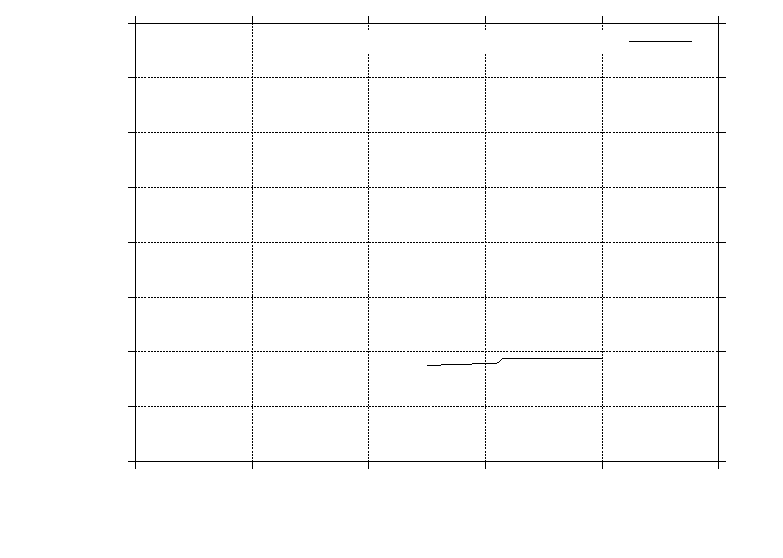
\includegraphics{E0ddepend}}%
    \gplfronttext
  \end{picture}%
\endgroup
  
\caption{The ground state free energy for $T = 0$, $E_0 + 2\mu N_F$, is plotted as a function of the interwire distance $d$. Black dashed: intrawire pairing only. Black dash-dotted: interwire pairing only. In red: $\Delta^{12}_k$ imaginary. In blue: $\Delta^{12}_k$ real. For the free gas: $(E_0 + 2\mu N_F)/\epsilon_{F,0}N_F = 2/3 = 0.667$. Parameters: $(n_Ba_B^3)^{1/3} = 0.01$, $(n_Ba_{BF}^3)^{1/3} = 0.11$, $l_t = 0$, $\frac{m_B}{m_F} = 7/40$, $\frac{n_F}{n_B^{1/3}} = 0.215$, $v_F/c_0 = 0.33$. }  
\label{fig.2wiresE0ddepend}  

% GNUPLOT: LaTeX picture with Postscript
\begingroup
  \makeatletter
  \providecommand\color[2][]{%
    \GenericError{(gnuplot) \space\space\space\@spaces}{%
      Package color not loaded in conjunction with
      terminal option `colourtext'%
    }{See the gnuplot documentation for explanation.%
    }{Either use 'blacktext' in gnuplot or load the package
      color.sty in LaTeX.}%
    \renewcommand\color[2][]{}%
  }%
  \providecommand\includegraphics[2][]{%
    \GenericError{(gnuplot) \space\space\space\@spaces}{%
      Package graphicx or graphics not loaded%
    }{See the gnuplot documentation for explanation.%
    }{The gnuplot epslatex terminal needs graphicx.sty or graphics.sty.}%
    \renewcommand\includegraphics[2][]{}%
  }%
  \providecommand\rotatebox[2]{#2}%
  \@ifundefined{ifGPcolor}{%
    \newif\ifGPcolor
    \GPcolorfalse
  }{}%
  \@ifundefined{ifGPblacktext}{%
    \newif\ifGPblacktext
    \GPblacktexttrue
  }{}%
  % define a \g@addto@macro without @ in the name:
  \let\gplgaddtomacro\g@addto@macro
  % define empty templates for all commands taking text:
  \gdef\gplbacktext{}%
  \gdef\gplfronttext{}%
  \makeatother
  \ifGPblacktext
    % no textcolor at all
    \def\colorrgb#1{}%
    \def\colorgray#1{}%
  \else
    % gray or color?
    \ifGPcolor
      \def\colorrgb#1{\color[rgb]{#1}}%
      \def\colorgray#1{\color[gray]{#1}}%
      \expandafter\def\csname LTw\endcsname{\color{white}}%
      \expandafter\def\csname LTb\endcsname{\color{black}}%
      \expandafter\def\csname LTa\endcsname{\color{black}}%
      \expandafter\def\csname LT0\endcsname{\color[rgb]{1,0,0}}%
      \expandafter\def\csname LT1\endcsname{\color[rgb]{0,1,0}}%
      \expandafter\def\csname LT2\endcsname{\color[rgb]{0,0,1}}%
      \expandafter\def\csname LT3\endcsname{\color[rgb]{1,0,1}}%
      \expandafter\def\csname LT4\endcsname{\color[rgb]{0,1,1}}%
      \expandafter\def\csname LT5\endcsname{\color[rgb]{1,1,0}}%
      \expandafter\def\csname LT6\endcsname{\color[rgb]{0,0,0}}%
      \expandafter\def\csname LT7\endcsname{\color[rgb]{1,0.3,0}}%
      \expandafter\def\csname LT8\endcsname{\color[rgb]{0.5,0.5,0.5}}%
    \else
      % gray
      \def\colorrgb#1{\color{black}}%
      \def\colorgray#1{\color[gray]{#1}}%
      \expandafter\def\csname LTw\endcsname{\color{white}}%
      \expandafter\def\csname LTb\endcsname{\color{black}}%
      \expandafter\def\csname LTa\endcsname{\color{black}}%
      \expandafter\def\csname LT0\endcsname{\color{black}}%
      \expandafter\def\csname LT1\endcsname{\color{black}}%
      \expandafter\def\csname LT2\endcsname{\color{black}}%
      \expandafter\def\csname LT3\endcsname{\color{black}}%
      \expandafter\def\csname LT4\endcsname{\color{black}}%
      \expandafter\def\csname LT5\endcsname{\color{black}}%
      \expandafter\def\csname LT6\endcsname{\color{black}}%
      \expandafter\def\csname LT7\endcsname{\color{black}}%
      \expandafter\def\csname LT8\endcsname{\color{black}}%
    \fi
  \fi
    \setlength{\unitlength}{0.0500bp}%
    \ifx\gptboxheight\undefined%
      \newlength{\gptboxheight}%
      \newlength{\gptboxwidth}%
      \newsavebox{\gptboxtext}%
    \fi%
    \setlength{\fboxrule}{0.5pt}%
    \setlength{\fboxsep}{1pt}%
\begin{picture}(7200.00,5040.00)%
    \gplgaddtomacro\gplbacktext{%
      \csname LTb\endcsname%
      \put(814,767){\makebox(0,0)[r]{\strut{}$0$}}%
      \csname LTb\endcsname%
      \put(814,1469){\makebox(0,0)[r]{\strut{}$0.1$}}%
      \csname LTb\endcsname%
      \put(814,2170){\makebox(0,0)[r]{\strut{}$0.2$}}%
      \csname LTb\endcsname%
      \put(814,2872){\makebox(0,0)[r]{\strut{}$0.3$}}%
      \csname LTb\endcsname%
      \put(814,3573){\makebox(0,0)[r]{\strut{}$0.4$}}%
      \csname LTb\endcsname%
      \put(814,4275){\makebox(0,0)[r]{\strut{}$0.5$}}%
      \csname LTb\endcsname%
      \put(814,4976){\makebox(0,0)[r]{\strut{}$0.6$}}%
      \csname LTb\endcsname%
      \put(1009,484){\makebox(0,0){\strut{}$0.71$}}%
      \csname LTb\endcsname%
      \put(1828,484){\makebox(0,0){\strut{}$0.72$}}%
      \csname LTb\endcsname%
      \put(2646,484){\makebox(0,0){\strut{}$0.73$}}%
      \csname LTb\endcsname%
      \put(3465,484){\makebox(0,0){\strut{}$0.74$}}%
      \csname LTb\endcsname%
      \put(4284,484){\makebox(0,0){\strut{}$0.75$}}%
      \csname LTb\endcsname%
      \put(5103,484){\makebox(0,0){\strut{}$0.76$}}%
      \csname LTb\endcsname%
      \put(5921,484){\makebox(0,0){\strut{}$0.77$}}%
      \csname LTb\endcsname%
      \put(6740,484){\makebox(0,0){\strut{}$0.78$}}%
    }%
    \gplgaddtomacro\gplfronttext{%
      \csname LTb\endcsname%
      \put(176,2871){\rotatebox{-270}{\makebox(0,0){\strut{}$Delta_k/epsilon_{F,0}$}}}%
      \put(3874,154){\makebox(0,0){\strut{}$k_Fd$}}%
      \csname LTb\endcsname%
      \put(3385,4803){\makebox(0,0)[r]{\strut{}$Intrawire pairing$}}%
      \csname LTb\endcsname%
      \put(3385,4583){\makebox(0,0)[r]{\strut{}$Interwire pairing$}}%
    }%
    \gplbacktext
    \put(0,0){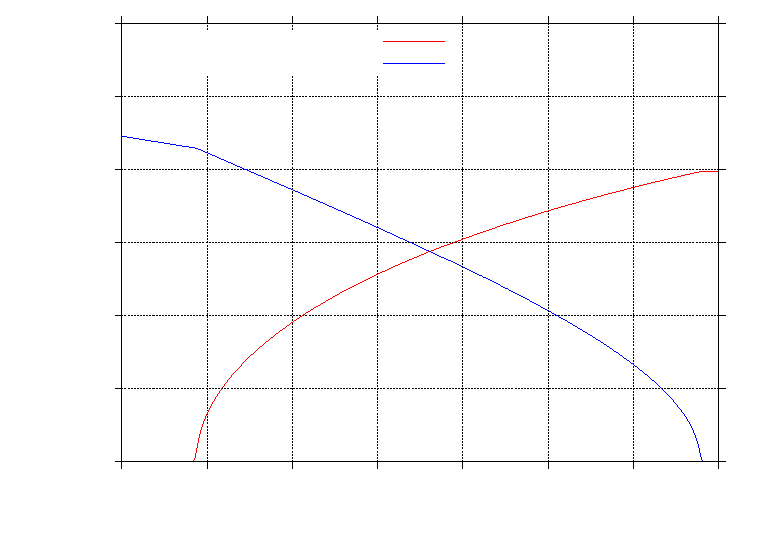
\includegraphics{ddepend}}%
    \gplfronttext
  \end{picture}%
\endgroup
  
\caption{The pairings at the Fermi momentum, $\left|\Delta^{11}_{k_F}\right|$ and $\left|\Delta^{12}_{k_F}\right|$, as a function of the distance $d$ between the wires. In red: pairings for $\Delta^{12}_k$ imaginary, corresponding to the red graph in figure \ref{fig.2wiresE0ddepend}. In blue: Pairings for $\Delta^{12}_k$ real, corresponding to the blue graph in figure \ref{fig.2wiresE0ddepend}. The \textit{inter}wire pairing is shown with dash-dotted lines. The \textit{intra}wire pairings are shown in solid. Parameters: $(n_Ba_B^3)^{1/3} = 0.01$, $(n_Ba_{BF}^3)^{1/3} = 0.11$, $l_t = 0$, $\frac{m_B}{m_F} = 7/40$, $\frac{n_F}{n_B^{1/3}} = 0.215$, $v_F/c_0 = 0.33$. }  
\label{fig.2wiresMaximalPairingddepend}  
\end{center}    
\end{figure}

Now let us concentrate on the energetically favourable solution: $\Delta^{12}_k$ imaginary. In this case the energy dispersions are identical and even in $k$: $E^{\pm}_{F,k} = E_{F,k} = \sqrt{\varepsilon_k^2 + (\Delta^{11}_k)^2 + |\Delta^{12}_k|^2}$. This means, that the gap equations in \eqref{eq.2wiresgapequations} partially decouples: 
\begin{align}
\Delta^{11}_k &= -\frac{1}{\mathcal{L}}\sum_{k'} W_{\text{ind}}^{11}(k, k')\frac{\Delta^{11}_{k'}}{2E_{F,k'}}\tanh\left(\frac{\beta E_{F,k'}}{2}\right), \nonumber \\
\Delta^{12}_k &= -\frac{1}{\mathcal{L}}\sum_{k'} W_{\text{ind}}^{12}(k, k')\frac{\Delta^{12}_{k'}}{2E_{F,k'}}\tanh\left(\frac{\beta E_{F,k'}}{2}\right).
\label{eq.2wiresgapequationsDelta12imaginary}
\end{align} 
This explicitly shows, that the two pairings are only coupled through the energy $E_{F,k}$. We start the analysis around $d = d_c$, since both pairings are suspected to be present there. For each value of $d$ we do something very similar to the above. However, here we do not reinitiate the initial guess in each step of $d$. In stead we reuse the found solution from the previous value of $d$. This makes the analysis much faster, and as long as the transition between the pairings is continuous no mistake is made. Further, we record the pairings at the Fermi momentum as above. The result is shown as the red curves in figure \ref{fig.2wiresMaximalPairingddepend}.
 
We see, that for small and large distances the expected behaviour is observed. Naively it seems to be the case, that the interwire pairing increases linearly for small $k_Fd$. However, an analysis to lower values of $d$ shows, that it diverges for $d \to 0$ as expected since the interwire interaction diverges in this limit. In between we see a continuous cross over region, where both pairings are present. Further, we notice that the intrawire pairing is constant from just under $k_Fd = 0.78$ and upwards as we expected. The fact that we start at $k_Fd = k_Fd_c = 0.748$, and then iterate downwards and upwards from there is the reason for the very small indent in the data precisely at this value. The figure only shows the pairing at $k_F$: $|\Delta_{k_F}|]$. We will return to the functional form of the pairings in chapter \ref{Chapter11}.

The combined result of the two figures tells us the following. We are able to find a cross over region of interwire distances $d$, where both an interwire $s$-wave pairing and an intrawire $p$-wave pairing is present, and this transition is the energetically favourable. The continuity of this solution fits with the topological analyses of sections \ref{sec.2wirestransitionqualitative} and \ref{sec.2wires_CSinv}. Further for the imaginary interwire pairing the sudden flip from intra- to interwire pairing means, that the gap closes precisely at $d = d_c$. However, it does so in a discontinuous way, which is \textit{not} required by the topology, as is evident again from sections \ref{sec.2wirestransitionqualitative} and \ref{sec.2wires_CSinv}. Hence, the numerical analysis shows, that we cannot \textit{only} rely on the topological analysis to get an idea of how the transition occures. There are key insights to gather from the numerical analysis. 


\section{Control of cross over through the coherence length}
\label{sec.2wires_crossover_control_coherence_length}
In this section we will investigate how we can control the cross over from intrawire to interwire pairing through the coherence length, $\xi$, of the Bose-Einstein condensate.

The range of the induced interaction is roughly the condensate coherence length:
\begin{equation}
k_F\frac{\xi}{\sqrt{2}} = \frac{\sqrt{\pi}}{4}\frac{1}{\sqrt{(n_Ba_B^3)^{1/3}}}\frac{n_F}{n_B^{1/3}}.
\label{eq.RangefunctionofrBBnB}
\end{equation}
We would like to explore the possibility of controlling the cross over through the coherence length. This is of experimental relevance. Adjusting the spatial distance, $d$, between the wires may be rather difficult in an experimental setup. If we can control an effective distance between the wires by adjusting the coherence length, this then might be a more realisable approach. We have the following intuitive idea of the feasibility of this approach. For a very short coherence length the induced interaction cannot reach across the distance $d$ between the wires. However, there is always a neighbour close by internally in the wire. Hence, we expect that for $\xi \to 0$ the system is in the intrawire pairing only regime. Opposite, for very long coherence lengths the distance between the wires becomes insignificant. Further, since the interwire induced interaction is enhanced by a factor of 2 relative to the intrawire one, we expect that for $\xi \to \infty$ the system enters the interwire pairing only regime. 

As mentioned in the end of chapter \ref{Chapter8}, we can quanitify this analysis in the following manner. We simply consider the transition as a competion of whether $\tilde{V}^{11}_{\text{ind}}(x,0)$ or $2\tilde{V}^{12}_{\text{ind}}(x,0)$ is the larger interaction. Explicitly, for some reference length $x_0$ we get the equation:
\begin{equation}
2 = \frac{ \tilde{V}^{11}_{\text{ ind }}(x_0, 0) }{ \tilde{V}^{12}_{\text{ ind }}(x_0, 0) } = \sqrt{ 1 + \left( \frac{ d_c }{ x_0 } \right)^2 }\text{ e }^{ -\frac{ \sqrt{2}x_0 }{ \xi } \left( 1 - \sqrt{ 1 + \left( \frac{ d_c }{ x_0 } \right)^2 } \right) }.
\label{eq.2wires.Vequal}
\end{equation}
For a specific value of $x_0$ we can solve this equation numerically. We will return to this shortly.  

For the numerical analysis based on the pairings, we will keep the Bose gas parameter $(n_Ba_B^3)^{1/3}$ constant and use the relative particle distance $n_F/n_B^{1/3}$ to vary the range of the interaction. This challenges the intuitive idea described above, because the induced interactions are both proportional to $n_B^{1/3}/n_F$. Hence, both decrease with an increase in the coherence length. 

The analysis is performed in the following way. We start at a high value of $n_F/n_B^{1/3}$. A direct and precise measure for the transition is the previously mentioned critical distance $d_c$. In practice this is found in the following way. First we calculate the free energy $F_1(\Delta^{11}_k) = E_0(\Delta^{11}_k) + 2 \mu (\Delta^{11}_k) N_F$ in the case, that there is only intrawire pairing, $\Delta^{11}_k$ present. This is independent of $d$ as described by the dashed curve in figure \ref{fig.2wiresE0ddepend}. Then we calculate the same, when only interwire pairing is present. We then iteratively find the value of $d = d_c$, where the free energies match: $F(\Delta^{12}_k, d_c) = F(\Delta^{11}_k)$. We then decrease $n_F/n_B^{1/3}$ by a small amount and repeat the process. The outcome of the analysis is shown as the black solid curve in figure \ref{fig.twowirescrossovernBdepend}. We notice, that $d_c$ exhibits a maximal value, and that it approaches a constant for large values of $n_F/n_B^{1/3}$. The dashed vertical line indicates where $v_F = c_0$. Therefore, the behaviour to the right of this line can only be considered as the zero frequency contribution. 

The area with white background indicates the \textit{intra}wire pairing only regime. The grey area is correspondingly \textit{inter}wire pairing only. We can understand this result in the following way. First, consider a constant value of the relative particle distance, e.g. $n_F/n_B^{1/3} = 0.2$. When we decrease the interwire distance from say $k_Fd = 1$ we move along the dashed vertical grid line at $n_F/n_B^{1/3} = 0.2$. The system experiences the cross over, when we cross the solid black line. This is as described in section \ref{sec.2wiresCrossover_energy}. Second, consider a constant value of the interwire distance, e.g. $k_Fd = 0.6$. When we increase $n_F/n_B^{1/3}$ we follow the horisontal grid line and the system again experiences the cross over, when it crosses the solid black line. 

\begin{figure} 
\begin{center}  
% GNUPLOT: LaTeX picture with Postscript
\begingroup
  \makeatletter
  \providecommand\color[2][]{%
    \GenericError{(gnuplot) \space\space\space\@spaces}{%
      Package color not loaded in conjunction with
      terminal option `colourtext'%
    }{See the gnuplot documentation for explanation.%
    }{Either use 'blacktext' in gnuplot or load the package
      color.sty in LaTeX.}%
    \renewcommand\color[2][]{}%
  }%
  \providecommand\includegraphics[2][]{%
    \GenericError{(gnuplot) \space\space\space\@spaces}{%
      Package graphicx or graphics not loaded%
    }{See the gnuplot documentation for explanation.%
    }{The gnuplot epslatex terminal needs graphicx.sty or graphics.sty.}%
    \renewcommand\includegraphics[2][]{}%
  }%
  \providecommand\rotatebox[2]{#2}%
  \@ifundefined{ifGPcolor}{%
    \newif\ifGPcolor
    \GPcolorfalse
  }{}%
  \@ifundefined{ifGPblacktext}{%
    \newif\ifGPblacktext
    \GPblacktexttrue
  }{}%
  % define a \g@addto@macro without @ in the name:
  \let\gplgaddtomacro\g@addto@macro
  % define empty templates for all commands taking text:
  \gdef\gplbacktext{}%
  \gdef\gplfronttext{}%
  \makeatother
  \ifGPblacktext
    % no textcolor at all
    \def\colorrgb#1{}%
    \def\colorgray#1{}%
  \else
    % gray or color?
    \ifGPcolor
      \def\colorrgb#1{\color[rgb]{#1}}%
      \def\colorgray#1{\color[gray]{#1}}%
      \expandafter\def\csname LTw\endcsname{\color{white}}%
      \expandafter\def\csname LTb\endcsname{\color{black}}%
      \expandafter\def\csname LTa\endcsname{\color{black}}%
      \expandafter\def\csname LT0\endcsname{\color[rgb]{1,0,0}}%
      \expandafter\def\csname LT1\endcsname{\color[rgb]{0,1,0}}%
      \expandafter\def\csname LT2\endcsname{\color[rgb]{0,0,1}}%
      \expandafter\def\csname LT3\endcsname{\color[rgb]{1,0,1}}%
      \expandafter\def\csname LT4\endcsname{\color[rgb]{0,1,1}}%
      \expandafter\def\csname LT5\endcsname{\color[rgb]{1,1,0}}%
      \expandafter\def\csname LT6\endcsname{\color[rgb]{0,0,0}}%
      \expandafter\def\csname LT7\endcsname{\color[rgb]{1,0.3,0}}%
      \expandafter\def\csname LT8\endcsname{\color[rgb]{0.5,0.5,0.5}}%
    \else
      % gray
      \def\colorrgb#1{\color{black}}%
      \def\colorgray#1{\color[gray]{#1}}%
      \expandafter\def\csname LTw\endcsname{\color{white}}%
      \expandafter\def\csname LTb\endcsname{\color{black}}%
      \expandafter\def\csname LTa\endcsname{\color{black}}%
      \expandafter\def\csname LT0\endcsname{\color{black}}%
      \expandafter\def\csname LT1\endcsname{\color{black}}%
      \expandafter\def\csname LT2\endcsname{\color{black}}%
      \expandafter\def\csname LT3\endcsname{\color{black}}%
      \expandafter\def\csname LT4\endcsname{\color{black}}%
      \expandafter\def\csname LT5\endcsname{\color{black}}%
      \expandafter\def\csname LT6\endcsname{\color{black}}%
      \expandafter\def\csname LT7\endcsname{\color{black}}%
      \expandafter\def\csname LT8\endcsname{\color{black}}%
    \fi
  \fi
    \setlength{\unitlength}{0.0500bp}%
    \ifx\gptboxheight\undefined%
      \newlength{\gptboxheight}%
      \newlength{\gptboxwidth}%
      \newsavebox{\gptboxtext}%
    \fi%
    \setlength{\fboxrule}{0.5pt}%
    \setlength{\fboxsep}{1pt}%
\begin{picture}(7200.00,5040.00)%
    \gplgaddtomacro\gplbacktext{%
    }%
    \gplgaddtomacro\gplfronttext{%
      \csname LTb\endcsname%
      \put(176,2871){\rotatebox{-270}{\makebox(0,0){\strut{}$k_Fd_c$}}}%
      \put(3874,154){\makebox(0,0){\strut{}$n_F/n_B^{1/3}$}}%
      \csname LTb\endcsname%
      \put(814,767){\makebox(0,0)[r]{\strut{}$0$}}%
      \csname LTb\endcsname%
      \put(814,1469){\makebox(0,0)[r]{\strut{}$0.2$}}%
      \csname LTb\endcsname%
      \put(814,2170){\makebox(0,0)[r]{\strut{}$0.4$}}%
      \csname LTb\endcsname%
      \put(814,2872){\makebox(0,0)[r]{\strut{}$0.6$}}%
      \csname LTb\endcsname%
      \put(814,3573){\makebox(0,0)[r]{\strut{}$0.8$}}%
      \csname LTb\endcsname%
      \put(814,4275){\makebox(0,0)[r]{\strut{}$1$}}%
      \csname LTb\endcsname%
      \put(814,4976){\makebox(0,0)[r]{\strut{}$1.2$}}%
      \csname LTb\endcsname%
      \put(1009,484){\makebox(0,0){\strut{}$0$}}%
      \csname LTb\endcsname%
      \put(1773,484){\makebox(0,0){\strut{}$0.2$}}%
      \csname LTb\endcsname%
      \put(2537,484){\makebox(0,0){\strut{}$0.4$}}%
      \csname LTb\endcsname%
      \put(3301,484){\makebox(0,0){\strut{}$0.6$}}%
      \csname LTb\endcsname%
      \put(4066,484){\makebox(0,0){\strut{}$0.8$}}%
      \csname LTb\endcsname%
      \put(4830,484){\makebox(0,0){\strut{}$1$}}%
      \csname LTb\endcsname%
      \put(5594,484){\makebox(0,0){\strut{}$1.2$}}%
      \csname LTb\endcsname%
      \put(6358,484){\makebox(0,0){\strut{}$1.4$}}%
      \put(1850,3924){\makebox(0,0)[l]{\strut{}Intrawire pairing only}}%
      \put(4142,2521){\makebox(0,0)[l]{\strut{}Interwire pairing only}}%
    }%
    \gplbacktext
    \put(0,0){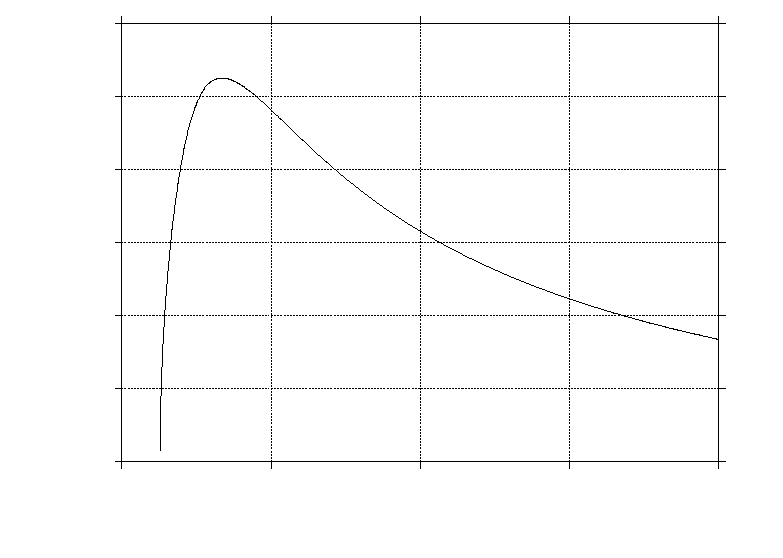
\includegraphics{Figures/twowires/Deltas3.1.3/nBdepend}}%
    \gplfronttext
  \end{picture}%
\endgroup
  
\caption{Solid line: the critical distance $d_c$ plotted as a function of the relative particle distance $n_F/n_B^{1/3}$. White background: intrawire pairing only regime. Grey background: interwire pairing only regime. Dash-dotted line: the critical distance according to the competition of intra- and interwire interactions for $k_Fx_0 = 1/\sqrt{3}$. See equation \eqref{eq.2wires.Vequal}. When we cross the solid line the system experiences the phase transition studied in section \ref{sec.2wiresCrossover_energy}. Dashed vertical line: $v_F = c_0$. The curve to the right hereof is only the zero frequency contribution. Parameters: $(n_Ba_B^3)^{1/3} = 0.01$, $(n_Ba_{BF}^3)^{1/3} = 0.11$, $l_t = 0$, $\frac{m_B}{m_F} = 7/40$. }  
\label{fig.twowirescrossovernBdepend}  
\end{center}    
\end{figure}

In this way we explicitly see, that instead of actually moving the wires we can control the cross over by adjusting $n_F/n_B^{1/3}$ and in turn the coherence length; see equation \eqref{eq.RangefunctionofrBBnB}. This all supports the intuitive idea outlined above. Caution should however be taken. Most importantly, there is an extremal value of $d_c$ at a finite value of $n_F/n_B^{1/3}$. Notice, that this also means, that just below this extremal value, there is an interval of distances, where the system experiences two cross overs. This is not explained by the competition of interactions. This we can see quite explicitly by solving equation \eqref{eq.2wires.Vequal} numerically. However, we have to choose a specific value of $x_0$. In the $\xi \to \infty$ limit we get a solvable form of the equation:
\begin{equation}
2 = \sqrt{1 + \left(\frac{d_c}{x_0}\right)^2} \Rightarrow d_c = \sqrt{3} x_0. \nonumber
\end{equation}
From this it is clear, that $d_c$ reaches a constant for $\xi \to \infty$ based on \eqref{eq.2wires.Vequal}. Hence, the fact that the actual critical distance $d_c$ has this asymptotic behaviour is well-described within a competition of interactions line of thinking. Further, in this line of thinking it is physically reasonable, that the asymptotic value of $d_c$ is the typical distance between the particles: $k_Fd_c = 1$.\footnote{This choice is reasonable, but not crucial. For any value of $x_0 > 0$ the result is the same.} Hence, we set $k_Fx_0 = 1/\sqrt{3}$. This results in the dash-dotted line in figure \ref{fig.twowirescrossovernBdepend}. From this it is clear, that the competition of interactions is not able to capture the fact, that the dependence of the critical distance, $d_c$, on the relative particle distance, $n_F/n_B^{1/3}$, is \textit{not} monotonic, but rather has a maximal value at a finite value of $n_F/n_B^{1/3}$ as mentioned above. This emphasizes the fact, that although a lot of physical intuition can be build on the form and behaviour of the interactions, we have to be careful when used to argue for the response of the system.

Let us try to understand this from a functional point of view instead. The intrawire pairing, $\Delta^{11}_k$, depends on the parameters $\beta, m_B/m_F, (n_Ba_B^3)^{1/3}$ and $n_B^{1/3}/n_F$ and is a functional of the pairings themselves: $\Delta^{11}_k, \Delta^{12}_k$. This is similarly the case for the interwire pairing, $\Delta^{12}_k$, with the additional parameter $d$. Hence, we can write:
\begin{equation}
\Delta^{11}_k = G\left(\Delta^{11}_k, \Delta^{12}_k, \beta, \frac{m_B}{m_F}, (n_Ba_B^3)^{1/3}, \frac{n_B^{1/3}}{n_F} \right), \hspace{0.5cm} \Delta^{12}_k = H\left(\Delta^{11}_k, \Delta^{12}_k, \beta, \frac{m_B}{m_F}, (n_Ba_B^3)^{1/3}, \frac{n_B^{1/3}}{n_F}, d \right), \nonumber 
\end{equation}
where $G$ and $H$ are the described functionals. On unitless form the functionals have a common prefactor, that depends on the mass ratio, the Bose gas parameter and the relative particle distance: $m_B/m_F, (n_Ba_B^3)^{1/3}$, and $n_B^{1/3}/n_F$. This means, that the limit of $n_F/n_B^{1/3} \to \infty $ is well-defined for the ratio of the pairings:
\begin{equation}
\lim_{\frac{n_F}{n_B^{1/3}} \to \infty} \left[\frac{|\Delta^{11}_{k_F}|]}{|\Delta^{12}_{k_F}|}\right] = \frac{\left|G\left(\Delta^{11}_{k_F}, \Delta^{12}_{k_F}, \beta, \frac{m_B}{m_F}, (n_Ba_B^3)^{1/3}, \frac{n_B^{1/3}}{n_F} = 0 \right)\right|}{\left|H\left(\Delta^{11}_{k_F}, \Delta^{12}_{k_F}, \beta, \frac{m_B}{m_F}, (n_Ba_B^3)^{1/3}, \frac{n_B^{1/3}}{n_F} = 0, d \right)\right|}. \nonumber
\end{equation}
Since the pairings at $k_F$ must be comparable at a distance similar to $d_c$, the above ratio will be equal to 1 at a distance similar to $d_c$. It is therefore evident that $d_c$ is independent of the relative particle distance for $n_F/n_B^{1/3} \gg 1$. Hence, $d_c$ must approach a constant for increasing values of $n_F/n_B^{1/3}$. 

The appearance of a maximum in $d_c$ can qualitatively be understood in the following way. For low values of $n_F/n_B^{1/3}$ the Bose gas becomes more rigid, since the spacing between the bosons becomes smaller. Hence, the wires must be brought closer together for the interwire pairing to dominate. For high values of $n_F/n_B^{1/3}$ the Bose gas is depleted. This means, that there are simply fewer bosons for the fermions to interact with. It is therefore reasonable, that $d_c$ should not exhibit a maximal value for $n_F/n_B^{1/3} \to \infty$. As a consequence a maximal value of $d_c$ appeares. This analysis is reminiscent of the analysis explaning the appearance of a minimum in the intrawire effective interaction, $W_\text{ind}^{11}(k_F,k_F)$, as a function of $n_F/n_B^{1/3}$. See subsection \ref{subsec.relevantmomenta.effectiveinteraction} for the details.  